%!TEX TS-program = xelatex
%!TEX encoding = UTF-8 Unicode
% Awesome CV LaTeX Template for CV/Resume
%
% This template has been downloaded from:
% https://github.com/posquit0/Awesome-CV
%
% Author:
% Claud D. Park <posquit0.bj@gmail.com>
% http://www.posquit0.com
%
%
% Adapted to be an Rmarkdown template by Mitchell O'Hara-Wild
% 23 November 2018
%
% Template license:
% CC BY-SA 4.0 (https://creativecommons.org/licenses/by-sa/4.0/)
%
%-------------------------------------------------------------------------------
% CONFIGURATIONS
%-------------------------------------------------------------------------------
% A4 paper size by default, use 'letterpaper' for US letter
\documentclass[11pt, a4paper]{awesome-cv}

% Configure page margins with geometry
\geometry{left=1.4cm, top=.8cm, right=1.4cm, bottom=1.8cm, footskip=.5cm}

% Specify the location of the included fonts
\fontdir[fonts/]

% Color for highlights
% Awesome Colors: awesome-emerald, awesome-skyblue, awesome-red, awesome-pink, awesome-orange
%                 awesome-nephritis, awesome-concrete, awesome-darknight

\definecolor{awesome}{HTML}{009ACD}

% Colors for text
% Uncomment if you would like to specify your own color
% \definecolor{darktext}{HTML}{414141}
% \definecolor{text}{HTML}{333333}
% \definecolor{graytext}{HTML}{5D5D5D}
% \definecolor{lighttext}{HTML}{999999}

% Set false if you don't want to highlight section with awesome color
\setbool{acvSectionColorHighlight}{true}

% If you would like to change the social information separator from a pipe (|) to something else
\renewcommand{\acvHeaderSocialSep}{\quad\textbar\quad}

\def\endfirstpage{\newpage}

%-------------------------------------------------------------------------------
%	PERSONAL INFORMATION
%	Comment any of the lines below if they are not required
%-------------------------------------------------------------------------------
% Available options: circle|rectangle,edge/noedge,left/right

\name{Buckminster}{Fuller}

\position{Architect \textgreater\textgreater{} Inventor
\textgreater\textgreater{} Futurist}
\address{407 S. Forest Ave., Carbondale, Illinois}

\mobile{+49 111 2222 3333}
\email{\href{mailto:buckminster.fuller@geodesic-mail.com}{\nolinkurl{buckminster.fuller@geodesic-mail.com}}}
\github{bucky1895}
\twitter{bucky1895}

% \gitlab{gitlab-id}
% \stackoverflow{SO-id}{SO-name}
% \skype{skype-id}
% \reddit{reddit-id}

\quote{When I am working on a problem, I never think about beauty but
when I have finished, if the solution is not beautiful, I know it is
wrong. We are called to be architects of the future, not its victims.
There is nothing in a caterpillar that tells you it's going to be a
butterfly. Love is metaphysical gravity. Don't fight forces, use them.
Integrity is the essence of everything successful. Everyone is born a
genius, but the process of living de-geniuses them.}

\usepackage{booktabs}

\providecommand{\tightlist}{%
	\setlength{\itemsep}{0pt}\setlength{\parskip}{0pt}}

%------------------------------------------------------------------------------


\usepackage{float} \usepackage{multicol} \usepackage{colortbl}

\arrayrulecolor{white}

\usepackage{hhline} \usepackage{fontawesome5}

\definecolor{light-gray}{gray}{0.95}

% Pandoc CSL macros
\newlength{\cslhangindent}
\setlength{\cslhangindent}{1.5em}
\newlength{\csllabelwidth}
\setlength{\csllabelwidth}{3em}
\newenvironment{CSLReferences}[3] % #1 hanging-ident, #2 entry spacing
 {% don't indent paragraphs
  \setlength{\parindent}{0pt}
  % turn on hanging indent if param 1 is 1
  \ifodd #1 \everypar{\setlength{\hangindent}{\cslhangindent}}\ignorespaces\fi
  % set entry spacing
  \ifnum #2 > 0
  \setlength{\parskip}{#2\baselineskip}
  \fi
 }%
 {}
\usepackage{calc}
\newcommand{\CSLBlock}[1]{#1\hfill\break}
\newcommand{\CSLLeftMargin}[1]{\parbox[t]{\csllabelwidth}{#1}}
\newcommand{\CSLRightInline}[1]{\parbox[t]{\linewidth - \csllabelwidth}{#1}}
\newcommand{\CSLIndent}[1]{\hspace{\cslhangindent}#1}

\begin{document}

% Print the header with above personal informations
% Give optional argument to change alignment(C: center, L: left, R: right)
\makecvheader

% Print the footer with 3 arguments(<left>, <center>, <right>)
% Leave any of these blank if they are not needed
% 2019-02-14 Chris Umphlett - add flexibility to the document name in footer, rather than have it be static Curriculum Vitae
\makecvfooter
  {August 2021}
    {Buckminster Fuller~~~·~~~Resume}
  {\thepage}


%-------------------------------------------------------------------------------
%	CV/RESUME CONTENT
%	Each section is imported separately, open each file in turn to modify content
%------------------------------------------------------------------------------



\hypertarget{my-journey}{%
\section{\texorpdfstring{\faIcon{plane} My
journey}{ My journey}}\label{my-journey}}

\begin{center}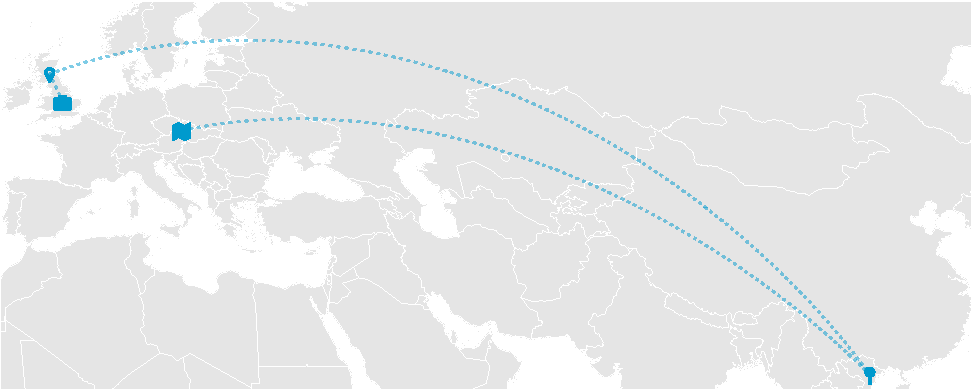
\includegraphics{DataDrivenResume_files/figure-latex/edu_plot-1} \end{center}

\begin{geoentries}

\georow{\geoentry{\faSuitcase}{Leicester, UK}{2000 - 2011}{attended Milton Academy in Massachusetts;began studying at Harvard College;was expelled from Harvard twice;worked as a mechanic in a textile mill;worked as a laborer in the meat-packing industry}}{\geoentry{\faMapMarker}{Edinburgh, UK}{2011 - 2015}{served in the U.S. Navy in World War I;worked as a shipboard radio operator;worked as an editor of a publication;worked as commander of the crash rescue boat USS Inca;acquired management experience in the meat-packing industry}}

\georow{\geoentry{\faMapPin}{Hanoi, VN}{2015 - 2017}{married Anne Hewlett;developed the Stockade Building System for fireproof housing;experienced a profound incident that I belong to the Universe;profoundly re-examinated my life;resolved to think independently}}{\geoentry{\faMap}{Brno, CZ}{2016 - Present Day}{committed to search for the principles governing the universe;accepted a job decorating the interior of the café Romany Marie's;worked in exchange for meals;gave informal lectures at the cafe several times a week;reinvented the geodesic dome}}

\end{geoentries}

\begin{geoentries}

\georow{\hypertarget{interests}{\section{\texorpdfstring{\faIcon{cog} Interests}{ Interests}}\label{interests}}}{\hypertarget{skills}{\section{\texorpdfstring{\faIcon{brain} Skills}{ Skills}}\label{skills}}}

\end{geoentries}

\vspace{-0.5cm}

\begin{center}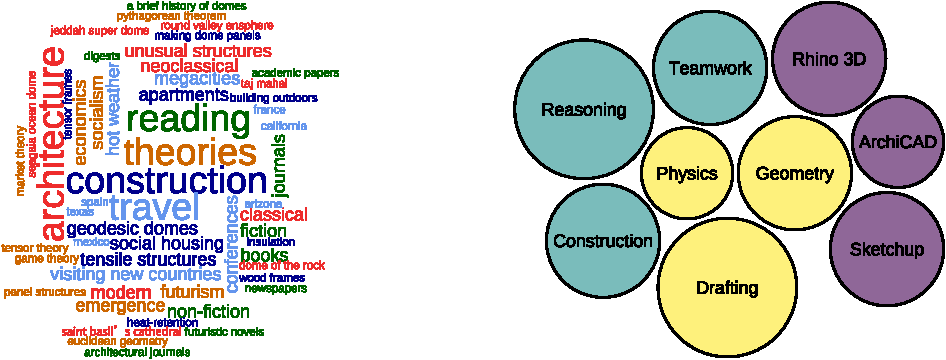
\includegraphics{DataDrivenResume_files/figure-latex/unnamed-chunk-15-1} \end{center}

\newpage

\hypertarget{selected-timeline}{%
\section{\texorpdfstring{\faIcon{user-clock} Selected
Timeline}{ Selected Timeline}}\label{selected-timeline}}

\begin{cventries}

\cventry{Specialisation in Dome Theory}{\faGraduationCap}{Brno, CZ}{Black Mountain College}{EDUCATION}{May 2021 - Aug 2021}{employed by the Marines to make small domes;
constructed first "continuous tension – discontinuous compression" geodesic dome at the University of Oregon}

\cventry{Higher Dipoloma Spanish Language}{\faGraduationCap}{Brno, CZ}{Brno Technical College}{EDUCATION}{Sep 2019 - Sep 2020}{served as a research professor of 'design science exploration' at the Southern Illinois University;
promoted to university professor in 1968 and distinguished university professor in 1972}

\cventry{PhD in Geodesic Domes (with scholarship)}{\faGraduationCap}{Brno, CZ}{North Carolina State University}{EDUCATION}{Jan 2019 - Aug 2021}{documented my life, philosophy and ideas scrupulously by a daily diary;
financed some of my experiments with inherited funds}

\cventry{Coordinator}{\faHandsHelping}{}{}{EXTRACURRICULAR}{Aug 2018 - Present Day}{inaugurated the World Design Science Decade (1965 to 1975) at the meeting of the International Union of Architects in Paris;
held a joint appointment at Southern Illinois University;
held a joint fellowship at a consortium of Philadelphia-area institutions, including the University of Pennsylvania}

\cventry{Volunteer}{\faHandsHelping}{}{}{EXTRACURRICULAR}{Jan 2016 - Mar 2019}{worked as a designer, scientist, developer, and writer including lecturing for many years around the world;
collaborated at SIU with John McHale}

\cventry{Event Organiser}{\faHandsHelping}{}{}{EXTRACURRICULAR}{Apr 2015 - Jun 2017}{appointed by University of Pennsylvania as university professor emeritus in 1975;
named as the 1969 Humanist of the Year by the American Humanist Association;
key participant at UN Habitat I, the first UN forum on human settlements}

\cventry{Master's Degree in Architecture}{\faGraduationCap}{Edinburgh, UK}{North Carolina State University}{EDUCATION}{Feb 2011 - Dec 2015}{successfully built huge geodesic domes during the 1950s;
lectured at North Carolina State University in Raleigh in 1949}

\cventry{Master Dome Builder}{\faBriefcase}{Leicester, UK}{Southern Illinois University}{EXPERIENCE}{Apr 2010 - Mar 2011}{taught at Black Mountain College in North Carolina during the summers of 1948 and 1949;
served as its Summer Institute director in 1949}

\cventry{BA in Architecture (First Class Honours)}{\faGraduationCap}{Leicester, UK}{University of California}{EDUCATION}{Sep 2007 - Dec 2010}{licensed ability to design geodesic domes to Geodesics, Inc. and Synergetics, Inc;
helped by Richard Lewontin to devise computer calculations for the lengths of the domes' edges}

\cventry{Certificate in Business Economics}{\faGraduationCap}{Leicester, UK}{Illinois Evening School}{EDUCATION}{Sep 2005 - Jun 2006}{co-founded the architectural firm Fuller \& Sadao Inc. in 1964 with architect Shoji Sadao;
designed the large geodesic dome for the U.S. Pavilion at Expo 67 in Montreal}

\cventry{Performer and Speaker}{\faBriefcase}{Leicester, UK}{California State Theater}{EXPERIENCE}{Mar 2001 - Aug 2009}{participated in a theatrical performance of Erik Satie's Le piège de Méduse produced by John Cage;
broke through my inhibitions to become confident as a performer and speaker}

\cventry{Sign Painter}{\faBriefcase}{Leicester, UK}{Self-Employed}{EXPERIENCE}{Mar 2001 - Oct 2008}{reinvented the geodesic dome;
constructed early model in 1945 at Bennington College in Vermont}

\cventry{Chief Executive Officer}{\faBriefcase}{Leicester, UK}{Geodesics Inc.}{EXPERIENCE}{Jan 2000 - Feb 2004}{erected a geodesic dome building that could sustain its own weight with no practical limits;
suspended several students from the structure's framework
started company Geodesics, Inc.}

\end{cventries}

\end{document}
